\section*{Supplementary information}
\renewcommand{\thetable}{S\arabic{table}}
\renewcommand{\thefigure}{S\arabic{figure}}
\setcounter{table}{0}
\setcounter{figure}{0}

\subsection*{S1. File identities}
\begin{table}[H]
\centering\scriptsize
\caption{SHA-256 hashes of the files that fix the analysis. The study runner recomputes the plan and addendum hashes at launch and records them in \texttt{results/study/primary/study.json}; both matched. Hashes of downloaded data files (MD5, as published by Zenodo) are in \texttt{docs/data\_sources.md} and each dataset's \texttt{download.json}.}
\label{tab:hashes}
\begin{tabular}{ll}
\toprule
File & SHA-256 \\
\midrule
\texttt{docs/analysis\_plan.md} & \texttt{602693ec8bead09526c51498a22588a5ab3cc24ceaf9943b402b4f55bad273cc} \\
\texttt{docs/analysis\_plan\_addendum.md} & \texttt{48d36c4965da3155e3adb6fdfd14c2a83eaee64ba518643aaccbe4307bfce054} \\
\texttt{configs/study.yaml} & \texttt{b762a26d9610a8c88d5111a48807447a24110402fbe3d519e10d09e99c51b71c} \\
\texttt{configs/benchmark\_norman.yaml} & \texttt{4ebdd9199f9d4d4216da69b0cd7aa32b94d27f13d8edaf916d9e93603321e618} \\
\texttt{requirements-lock.txt} & \texttt{a5336ce52ab9b2cb11d251805b47eb7801917db72a41e67cf0bd08c3b73a3944} \\
\bottomrule
\end{tabular}
\end{table}

\subsection*{S2. Hyperparameters and seeds}
\begin{table}[H]
\centering\scriptsize
\caption{Settings used in every dataset (from \texttt{configs/benchmark\_norman.yaml} and \texttt{configs/study.yaml}). Hyperparameters marked ``selected'' were chosen per fold on the calibration genes by masked MSE.}
\label{tab:grids}
\begin{tabularx}{\linewidth}{lX}
\toprule
Component & Setting \\
\midrule
Preprocessing & $10^4$ counts per cell, log1p; 2{,}000 genes by binned dispersion in control cells (20 bins, detection $\ge1\%$) plus targets; $\ge50$ cells per condition (25 fallback); co-expression embedding 32 dimensions from $\le$8{,}000 control cells \\
Splits & 5 folds over target genes, fold seed 0 (robustness seeds 1--3); 15\% of remaining genes for calibration \\
Ridge & $\alpha\in\{0.1,1,10,100,1000,10000\}$, selected; features standardised on training conditions \\
Gene-loading ridge & 10 principal components of the training residual matrix; $\alpha$ as ridge, selected \\
kNN & $k\in\{1,3,5,10\}$, selected; neighbours among conditions with the same number of targets \\
Bootstrap ridge & 8 bootstrap members; $\alpha$ selected as ridge \\
MLP ensemble & 5 members, each on a bootstrap resample, member seed $1000m$; hidden layers 128 and 64 (ReLU), dropout 0.1; output 20 PCA components of training residuals; Huber loss ($\delta=1$); AdamW, learning rate $10^{-3}$, weight decay $10^{-3}$, batch 32; at most 400 epochs, early stopping with patience 40 on calibration loss \\
Intervals & 90\% per-gene, split-conformal style on calibration-gene residuals; per-gene scale = median absolute residual, floored at 10\% of the median scale \\
Ranking & top 20\% of held-out perturbations by predicted RMS response \\
\bottomrule
\end{tabularx}
\end{table}

\subsection*{S3. Discovery benchmark on Norman 2019}
The discovery benchmark trained on single genes and pairs together and evaluated three held-out strata in the unseen-gene task, plus pairs whose singles were measured (Table~\ref{tab:discovery}). These analyses informed the models, baselines and metrics in the analysis plan. Scaled additive, additive plus mean residual, singles-only models, the non-additive and top-gene coverage metrics, and the pair-ranking analyses were all added after first results on these same folds. Their discovery estimates are therefore optimistic in an unknown direction and are not confirmatory.

\begin{table}[H]
\centering\scriptsize
\caption{Discovery benchmark (Norman 2019; 5 folds, seed 0). Models trained with pairs and singles. Skill is relative to the training mean; $r$, specific is the correlation of deviations from it. In the confirmation study, models were trained on single-gene conditions only, which changes the unseen-single results (main text).}
\label{tab:discovery}
\begin{tabular}{llccr}
\toprule
Stratum & Model & Skill vs mean (95\% CI) & $r$, specific & $n$ \\
\midrule
Pair, both singles measured & mlp\_on\_additive & 0.629 (0.588, 0.666) & 0.832 & 127 \\
 & ridge\_on\_additive & 0.622 (0.581, 0.660) & 0.828 & 127 \\
 & bootstrap\_ridge\_on\_additive & 0.615 (0.572, 0.653) & 0.825 & 127 \\
 & scaled\_additive & 0.598 (0.555, 0.638) & 0.790 & 127 \\
 & knn\_on\_additive & 0.597 (0.539, 0.648) & 0.822 & 127 \\
 & additive\_plus\_mean\_residual & 0.535 (0.478, 0.589) & 0.810 & 127 \\
 & additive & 0.485 (0.415, 0.548) & 0.796 & 127 \\
 & mlp\_ensemble & 0.404 (0.348, 0.460) & 0.655 & 127 \\
 & ridge & 0.222 (0.147, 0.289) & 0.516 & 127 \\
 & knn & 0.182 (0.097, 0.261) & 0.487 & 127 \\
 & bootstrap\_ridge & 0.181 (0.095, 0.261) & 0.498 & 127 \\
 & gene\_loading\_ridge & 0.078 (0.038, 0.116) & 0.260 & 127 \\
 & ridge\_singles\_only & 0.055 (-0.012, 0.116) & 0.319 & 127 \\
 & mean & 0.000 (0.000, 0.000) & -- & 127 \\
 & gene\_loading\_singles\_only & -0.079 (-0.132, -0.029) & 0.080 & 127 \\
Pair, one gene unseen & mlp\_ensemble & 0.071 (0.033, 0.108) & 0.309 & 100 \\
 & ridge & 0.051 (0.018, 0.082) & 0.291 & 100 \\
 & bootstrap\_ridge & 0.042 (0.011, 0.073) & 0.268 & 100 \\
 & gene\_loading\_ridge & 0.004 (-0.018, 0.022) & 0.127 & 100 \\
 & mean & 0.000 (0.000, 0.000) & -- & 100 \\
 & ridge\_singles\_only & -0.008 (-0.064, 0.044) & 0.175 & 100 \\
 & gene\_loading\_singles\_only & -0.017 (-0.075, 0.037) & 0.165 & 100 \\
 & knn & -0.031 (-0.101, 0.040) & 0.240 & 100 \\
Unseen single gene & mean & 0.000 (0.000, 0.000) & -- & 105 \\
 & gene\_loading\_singles\_only & -0.003 (-0.007, 0.001) & 0.028 & 105 \\
 & ridge\_singles\_only & -0.003 (-0.010, 0.003) & 0.016 & 105 \\
 & gene\_loading\_ridge & -0.018 (-0.037, -0.003) & 0.022 & 105 \\
 & ridge & -0.124 (-0.234, -0.038) & 0.051 & 105 \\
 & bootstrap\_ridge & -0.127 (-0.226, -0.046) & 0.024 & 105 \\
 & mlp\_ensemble & -0.175 (-0.306, -0.062) & 0.062 & 105 \\
 & knn & -0.288 (-0.372, -0.202) & -0.029 & 105 \\
\bottomrule
\end{tabular}
\end{table}

\subsection*{S4. Robustness to the fold partition}
Pre-specified analysis D4 repeated the unseen-gene task with three further fold partitions (Table~\ref{tab:seeds}).

\begin{table}[H]
\centering\scriptsize
\caption{Mean skill relative to the training mean on held-out genes, for four fold partitions. Seed 0 is the primary analysis.}
\label{tab:seeds}
\begin{tabular}{llrrrr}
\toprule
Dataset & Model & Seed 0 & Seed 1 & Seed 2 & Seed 3 \\
\midrule
Norman K562 CRISPRa & Gene-loading ridge & -0.003 & -0.009 & -0.007 & -0.001 \\
Norman K562 CRISPRa & MLP ensemble & -0.006 & -0.012 & -0.013 & -0.003 \\
Norman K562 CRISPRa & Ridge & -0.003 & -0.006 & -0.001 & -0.001 \\
Replogle K562 CRISPRi & Gene-loading ridge & 0.018 & 0.008 & 0.014 & 0.012 \\
Replogle K562 CRISPRi & MLP ensemble & 0.051 & 0.045 & 0.051 & 0.050 \\
Replogle K562 CRISPRi & Ridge & 0.025 & 0.024 & 0.020 & 0.026 \\
Replogle RPE1 CRISPRi & Gene-loading ridge & 0.010 & 0.004 & 0.006 & 0.008 \\
Replogle RPE1 CRISPRi & MLP ensemble & 0.052 & 0.046 & 0.052 & 0.061 \\
Replogle RPE1 CRISPRi & Ridge & 0.011 & 0.002 & 0.008 & 0.010 \\
Tian neurons CRISPRa & Gene-loading ridge & -0.001 & -0.009 & -0.028 & -0.000 \\
Tian neurons CRISPRa & MLP ensemble & 0.012 & 0.007 & 0.009 & 0.017 \\
Tian neurons CRISPRa & Ridge & -0.010 & -0.008 & -0.001 & 0.001 \\
Tian neurons CRISPRi & Gene-loading ridge & -0.000 & -0.000 & -0.000 & 0.000 \\
Tian neurons CRISPRi & MLP ensemble & -0.001 & -0.001 & -0.000 & -0.000 \\
Tian neurons CRISPRi & Ridge & -0.000 & -0.000 & -0.000 & -0.000 \\
\bottomrule
\end{tabular}
\end{table}

\subsection*{S5. Distribution of per-perturbation differences behind C1 (post hoc)}
Figure~\ref{fig:c1dist} and Table~\ref{tab:c1med} show the full distribution of per-perturbation MSE differences, with the median alongside the mean. In the Replogle screens the median difference favours every model and the distributions are left-skewed: a minority of perturbations is predicted much better than by the mean. In Tian CRISPRa, the MLP is better for most perturbations, but a few large right-tail losses move the mean towards zero (main text).

\begin{figure}[H]
\centering
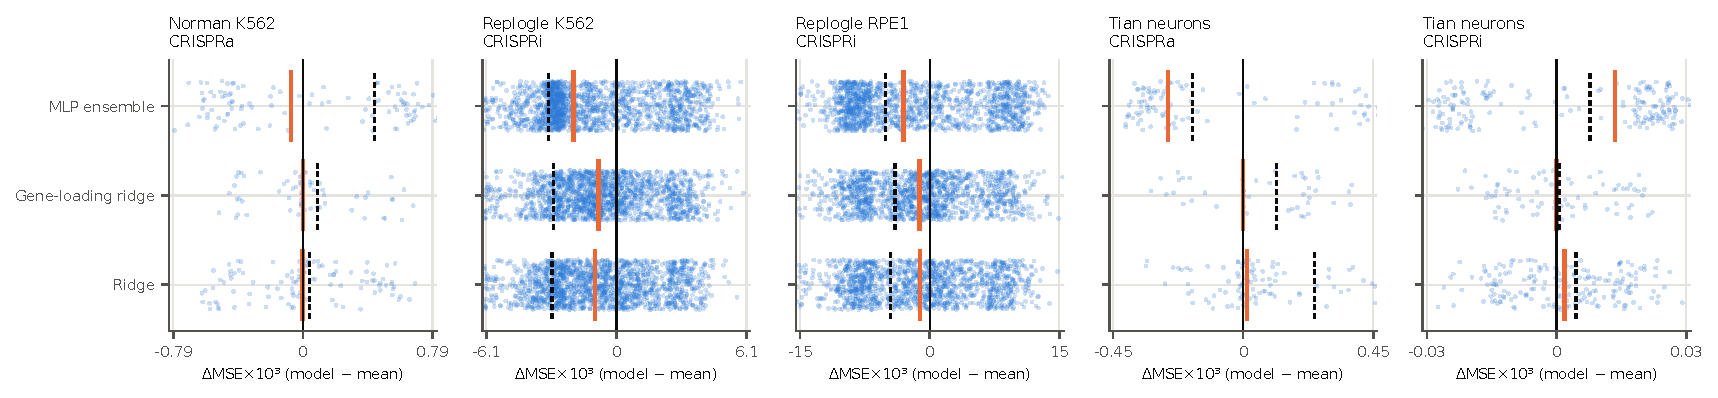
\includegraphics[width=\linewidth]{figures/figS1_c1_distribution.pdf}
\caption{Per-perturbation difference in MSE between each model and the mean baseline (negative favours the model), on a symmetric-log axis. Each point is one held-out gene. Orange: median; dashed black: mean.}
\label{fig:c1dist}
\end{figure}

\begin{table}[H]
\centering\scriptsize
\caption{Mean and median per-perturbation $\Delta$MSE $\times10^3$ (model $-$ mean), with bootstrap 95\% intervals for the median, and the fraction of perturbations on which the model is better.}
\label{tab:c1med}
\resizebox{0.9\linewidth}{!}{\begin{tabular}{llrcr}
\toprule
Dataset & Model & Mean $\Delta$MSE$\times10^3$ & Median (95\% CI) & Model better \\
\midrule
Norman K562 CRISPRa & Ridge & +0.004 & -0.000 (-0.005, +0.006) & 51\% \\
Norman K562 CRISPRa & Gene-loading ridge & +0.008 & -0.000 (-0.000, +0.000) & 50\% \\
Norman K562 CRISPRa & MLP ensemble & +0.061 & -0.007 (-0.031, +0.041) & 51\% \\
Replogle K562 CRISPRi & Ridge & -0.231 & -0.050 (-0.059, -0.039) & 62\% \\
Replogle K562 CRISPRi & Gene-loading ridge & -0.214 & -0.042 (-0.047, -0.037) & 64\% \\
Replogle K562 CRISPRi & MLP ensemble & -0.274 & -0.101 (-0.109, -0.088) & 67\% \\
Replogle RPE1 CRISPRi & Ridge & -0.428 & -0.105 (-0.141, -0.046) & 56\% \\
Replogle RPE1 CRISPRi & Gene-loading ridge & -0.380 & -0.110 (-0.150, -0.075) & 59\% \\
Replogle RPE1 CRISPRi & MLP ensemble & -0.480 & -0.284 (-0.366, -0.199) & 60\% \\
Tian neurons CRISPRa & Ridge & +0.023 & +0.001 (+0.000, +0.002) & 38\% \\
Tian neurons CRISPRa & Gene-loading ridge & +0.005 & +0.000 (+0.000, +0.000) & 39\% \\
Tian neurons CRISPRa & MLP ensemble & -0.008 & -0.028 (-0.041, -0.019) & 71\% \\
Tian neurons CRISPRi & Ridge & +0.000 & +0.000 (-0.000, +0.000) & 43\% \\
Tian neurons CRISPRi & Gene-loading ridge & +0.000 & -0.000 (-0.000, +0.000) & 53\% \\
Tian neurons CRISPRi & MLP ensemble & +0.001 & +0.001 (-0.001, +0.003) & 45\% \\
\bottomrule
\end{tabular}}
\end{table}

\subsection*{S6. Feature ablation and control-cell check (post hoc)}
\begin{table}[H]
\centering\scriptsize
\caption{Skill on held-out single genes with different feature sets (primary folds, seed 0). The last column is the paired difference from the primary features with a 95\% bootstrap interval. ``Primary, training-half controls'' recomputes the co-expression embedding and both baseline features from the control cells that contribute only to training targets.}
\label{tab:ablation}
\resizebox{\linewidth}{!}{\begin{tabular}{lllcc}
\toprule
Dataset, model & Features & Skill (95\% CI) & $r$, specific & Skill $-$ primary (95\% CI) \\
\midrule
Norman K562 CRISPRa, Ridge & Co-expression + baseline (primary) & -0.003 (-0.010, 0.004) & 0.016 & -- \\
 & Co-expression only & -0.003 (-0.011, 0.004) & 0.015 & +0.000 (-0.001, +0.001) \\
 & Baseline mean + detection & -0.008 (-0.017, -0.000) & -0.016 & -0.005 (-0.016, +0.006) \\
 & Baseline mean only & -0.005 (-0.012, 0.000) & -0.008 & -0.002 (-0.011, +0.007) \\
 & Detection rate only & -0.007 (-0.018, 0.004) & -0.014 & -0.004 (-0.017, +0.010) \\
 & Primary, training-half controls & 0.002 (-0.000, 0.006) & 0.026 & +0.006 (-0.001, +0.013) \\
Norman K562 CRISPRa, MLP ensemble & Co-expression + baseline (primary) & -0.006 (-0.021, 0.009) & 0.042 & -- \\
 & Co-expression only & -0.014 (-0.026, -0.002) & -0.004 & -0.008 (-0.019, +0.004) \\
 & Baseline mean + detection & -0.008 (-0.022, 0.005) & 0.015 & -0.002 (-0.022, +0.016) \\
 & Baseline mean only & 0.001 (-0.013, 0.014) & 0.036 & +0.007 (-0.011, +0.024) \\
 & Detection rate only & 0.005 (-0.011, 0.021) & 0.045 & +0.011 (-0.010, +0.033) \\
 & Primary, training-half controls & -0.002 (-0.014, 0.010) & 0.017 & +0.004 (-0.012, +0.021) \\
Replogle K562 CRISPRi, Ridge & Co-expression + baseline (primary) & 0.025 (0.015, 0.034) & 0.164 & -- \\
 & Co-expression only & 0.020 (0.010, 0.029) & 0.161 & -0.005 (-0.008, -0.003) \\
 & Baseline mean + detection & 0.006 (-0.002, 0.014) & 0.092 & -0.019 (-0.026, -0.013) \\
 & Baseline mean only & 0.004 (-0.002, 0.011) & 0.075 & -0.021 (-0.028, -0.013) \\
 & Detection rate only & 0.000 (-0.003, 0.003) & 0.064 & -0.025 (-0.033, -0.016) \\
 & Primary, training-half controls & 0.024 (0.014, 0.033) & 0.164 & -0.001 (-0.003, +0.001) \\
Replogle K562 CRISPRi, MLP ensemble & Co-expression + baseline (primary) & 0.051 (0.037, 0.061) & 0.213 & -- \\
 & Co-expression only & 0.049 (0.035, 0.061) & 0.213 & -0.001 (-0.004, +0.001) \\
 & Baseline mean + detection & 0.033 (0.022, 0.042) & 0.161 & -0.018 (-0.027, -0.010) \\
 & Baseline mean only & 0.033 (0.022, 0.043) & 0.164 & -0.018 (-0.026, -0.010) \\
 & Detection rate only & 0.026 (0.018, 0.034) & 0.147 & -0.024 (-0.036, -0.013) \\
 & Primary, training-half controls & 0.052 (0.039, 0.062) & 0.212 & +0.001 (-0.002, +0.003) \\
Replogle RPE1 CRISPRi, Ridge & Co-expression + baseline (primary) & 0.011 (-0.003, 0.024) & 0.138 & -- \\
 & Co-expression only & 0.012 (-0.001, 0.025) & 0.141 & +0.001 (+0.000, +0.003) \\
 & Baseline mean + detection & -0.000 (-0.008, 0.007) & 0.073 & -0.011 (-0.022, +0.001) \\
 & Baseline mean only & 0.001 (-0.004, 0.006) & 0.080 & -0.010 (-0.022, +0.003) \\
 & Detection rate only & -0.004 (-0.007, -0.000) & 0.029 & -0.014 (-0.027, -0.001) \\
 & Primary, training-half controls & 0.015 (0.001, 0.027) & 0.134 & +0.004 (-0.001, +0.010) \\
Replogle RPE1 CRISPRi, MLP ensemble & Co-expression + baseline (primary) & 0.052 (0.037, 0.066) & 0.193 & -- \\
 & Co-expression only & 0.051 (0.036, 0.064) & 0.194 & -0.001 (-0.006, +0.005) \\
 & Baseline mean + detection & 0.035 (0.024, 0.045) & 0.160 & -0.017 (-0.030, -0.003) \\
 & Baseline mean only & 0.036 (0.023, 0.047) & 0.164 & -0.016 (-0.030, -0.002) \\
 & Detection rate only & 0.038 (0.030, 0.047) & 0.157 & -0.013 (-0.027, +0.000) \\
 & Primary, training-half controls & 0.048 (0.034, 0.062) & 0.194 & -0.003 (-0.012, +0.006) \\
Tian neurons CRISPRa, Ridge & Co-expression + baseline (primary) & -0.010 (-0.018, -0.003) & -0.041 & -- \\
 & Co-expression only & -0.009 (-0.018, -0.003) & -0.044 & +0.000 (-0.001, +0.001) \\
 & Baseline mean + detection & -0.003 (-0.006, 0.001) & 0.018 & +0.007 (-0.001, +0.016) \\
 & Baseline mean only & -0.001 (-0.002, -0.000) & -0.020 & +0.008 (+0.002, +0.017) \\
 & Detection rate only & -0.002 (-0.005, 0.001) & 0.028 & +0.008 (+0.000, +0.017) \\
 & Primary, training-half controls & -0.001 (-0.005, 0.003) & 0.002 & +0.009 (+0.001, +0.017) \\
Tian neurons CRISPRa, MLP ensemble & Co-expression + baseline (primary) & 0.012 (0.003, 0.020) & 0.094 & -- \\
 & Co-expression only & 0.007 (-0.001, 0.014) & 0.058 & -0.005 (-0.009, -0.000) \\
 & Baseline mean + detection & 0.019 (0.009, 0.029) & 0.114 & +0.007 (+0.002, +0.012) \\
 & Baseline mean only & 0.017 (0.005, 0.027) & 0.110 & +0.005 (-0.001, +0.010) \\
 & Detection rate only & 0.018 (0.009, 0.027) & 0.105 & +0.006 (+0.001, +0.011) \\
 & Primary, training-half controls & 0.017 (0.009, 0.025) & 0.107 & +0.005 (+0.000, +0.010) \\
Tian neurons CRISPRi, Ridge & Co-expression + baseline (primary) & -0.000 (-0.000, 0.000) & -0.000 & -- \\
 & Co-expression only & -0.000 (-0.000, 0.000) & 0.000 & +0.000 (-0.000, +0.000) \\
 & Baseline mean + detection & -0.000 (-0.000, 0.000) & -0.003 & +0.000 (-0.000, +0.000) \\
 & Baseline mean only & -0.000 (-0.000, -0.000) & 0.001 & -0.000 (-0.000, +0.000) \\
 & Detection rate only & -0.000 (-0.000, 0.000) & -0.005 & +0.000 (-0.000, +0.000) \\
 & Primary, training-half controls & -0.000 (-0.000, 0.000) & 0.007 & -0.000 (-0.000, +0.000) \\
Tian neurons CRISPRi, MLP ensemble & Co-expression + baseline (primary) & -0.001 (-0.001, 0.000) & 0.013 & -- \\
 & Co-expression only & -0.001 (-0.002, 0.000) & -0.000 & -0.000 (-0.001, +0.001) \\
 & Baseline mean + detection & -0.002 (-0.003, -0.001) & -0.007 & -0.001 (-0.002, -0.000) \\
 & Baseline mean only & -0.001 (-0.002, -0.000) & 0.008 & -0.001 (-0.001, +0.000) \\
 & Detection rate only & -0.002 (-0.003, -0.001) & -0.006 & -0.001 (-0.002, -0.000) \\
 & Primary, training-half controls & -0.001 (-0.002, -0.000) & 0.006 & -0.000 (-0.001, +0.000) \\
\bottomrule
\end{tabular}}
\end{table}

\subsection*{S7. Interval calibration stratified by predicted magnitude (post hoc)}
\begin{table}[H]
\centering\scriptsize
\caption{Coverage of nominal 90\% per-gene intervals on held-out single genes. ``Standard'' calibrates one quantile over all genes. ``Stratified'' calibrates it within five strata of predicted deviation from the training mean. Top-20 responders are each perturbation's 20 genes with the largest observed deviation. The width ratio compares the mean interval width on those genes (stratified / standard).}
\label{tab:intervals}
\begin{tabular}{llccccc}
\toprule
 & & \multicolumn{2}{c}{All genes} & \multicolumn{2}{c}{Top-20 responders} & Width ratio, \\
Dataset & Model & Standard & Stratified & Standard & Stratified & top-20 \\
\midrule
Norman K562 CRISPRa & Ridge & 0.86 & 0.86 & 0.46 & 0.48 & 1.0 \\
Norman K562 CRISPRa & MLP ensemble & 0.86 & 0.86 & 0.45 & 0.47 & 1.0 \\
Replogle K562 CRISPRi & Ridge & 0.90 & 0.90 & 0.34 & 0.36 & 1.0 \\
Replogle K562 CRISPRi & MLP ensemble & 0.90 & 0.90 & 0.35 & 0.37 & 1.0 \\
Replogle RPE1 CRISPRi & Ridge & 0.90 & 0.90 & 0.57 & 0.57 & 1.0 \\
Replogle RPE1 CRISPRi & MLP ensemble & 0.90 & 0.90 & 0.55 & 0.55 & 1.0 \\
Tian neurons CRISPRa & Ridge & 0.87 & 0.87 & 0.60 & 0.62 & 1.0 \\
Tian neurons CRISPRa & MLP ensemble & 0.88 & 0.88 & 0.59 & 0.62 & 1.1 \\
Tian neurons CRISPRi & Ridge & 0.89 & 0.89 & 0.69 & 0.70 & 1.0 \\
Tian neurons CRISPRi & MLP ensemble & 0.89 & 0.89 & 0.69 & 0.71 & 1.0 \\
\bottomrule
\end{tabular}
\end{table}

\subsection*{S8. Second-revision analyses (post hoc)}
All analyses in this section used a further preprocessing pass that reproduced every primary target exactly (maximum difference 0).

\begin{table}[H]
\centering\scriptsize
\caption{Technical reproducibility limits. Limits for the primary batch partition with 95\% bootstrap intervals over perturbations; range over five partitions of batches into two sets; limits from random cell halves; and the fraction of perturbations whose specific response reproduces ($r\ge0.5$) in the primary partition. Tian CRISPRa has two batches, so all its partitions are the same contrast.}
\label{tab:limits}
\resizebox{\linewidth}{!}{\begin{tabular}{lcccccc}
\toprule
Dataset & Batches & Distinct partitions & Limit, primary partition (95\% CI) & Range over partitions & Limit, cell halves (95\% CI) & Reproducible \\
\midrule
Norman K562 CRISPRa & 8 & 4 & 0.93 (0.92, 0.94) & 0.93--0.93 & 0.93 (0.92, 0.95) & 94\% \\
Replogle K562 CRISPRi & 48 & 5 & 0.72 (0.71, 0.73) & 0.72--0.72 & 0.72 (0.71, 0.73) & 33\% \\
Replogle RPE1 CRISPRi & 56 & 5 & 0.85 (0.85, 0.86) & 0.85--0.85 & 0.85 (0.84, 0.86) & 72\% \\
Tian neurons CRISPRa & 2 & 1 & 0.46 (0.41, 0.51) & 0.46--0.46 & 0.55 (0.51, 0.58) & 8\% \\
Tian neurons CRISPRi & 4 & 2 & 0.19 (0.16, 0.21) & 0.17--0.19 & 0.19 (0.17, 0.22) & 1\% \\
\bottomrule
\end{tabular}}
\end{table}

\begin{table}[H]
\centering\scriptsize
\caption{Duplicate win rates with 95\% Wilson intervals, against the mean of other perturbations and, separately, against a zero prediction.}
\label{tab:discrimination}
\begin{tabular}{llcc}
\toprule
Dataset & Metric & Duplicate vs mean (95\% CI) & Duplicate vs zero (95\% CI) \\
\midrule
Norman K562 CRISPRa & MSE & 0.94 (0.88, 0.97) & 0.93 (0.87, 0.97) \\
 & $r$ (raw) & 0.95 (0.89, 0.98) & 1.00 (0.96, 1.00) \\
 & $r$ (specific) & 1.00 (0.96, 1.00) & 0.93 (0.87, 0.97) \\
 & $\rho$ (specific) & 1.00 (0.96, 1.00) & 0.78 (0.69, 0.85) \\
 & Top-20 recall & 0.93 (0.87, 0.97) & 1.00 (0.96, 1.00) \\
Replogle K562 CRISPRi & MSE & 0.34 (0.32, 0.36) & 0.37 (0.35, 0.39) \\
 & $r$ (raw) & 0.80 (0.78, 0.82) & 0.97 (0.96, 0.97) \\
 & $r$ (specific) & 1.00 (0.99, 1.00) & 0.63 (0.60, 0.65) \\
 & $\rho$ (specific) & 1.00 (0.99, 1.00) & 0.57 (0.55, 0.60) \\
 & Top-20 recall & 0.84 (0.82, 0.85) & 0.92 (0.91, 0.94) \\
Replogle RPE1 CRISPRi & MSE & 0.72 (0.70, 0.75) & 0.60 (0.58, 0.63) \\
 & $r$ (raw) & 0.73 (0.70, 0.75) & 0.98 (0.97, 0.98) \\
 & $r$ (specific) & 1.00 (1.00, 1.00) & 0.66 (0.63, 0.68) \\
 & $\rho$ (specific) & 1.00 (0.99, 1.00) & 0.60 (0.58, 0.63) \\
 & Top-20 recall & 0.75 (0.73, 0.77) & 0.97 (0.96, 0.97) \\
Tian neurons CRISPRa & MSE & 0.12 (0.07, 0.20) & 0.12 (0.07, 0.20) \\
 & $r$ (raw) & 0.82 (0.74, 0.89) & 0.77 (0.68, 0.85) \\
 & $r$ (specific) & 1.00 (0.96, 1.00) & 0.15 (0.10, 0.24) \\
 & $\rho$ (specific) & 1.00 (0.96, 1.00) & 0.10 (0.06, 0.18) \\
 & Top-20 recall & 0.46 (0.37, 0.56) & 0.94 (0.87, 0.97) \\
Tian neurons CRISPRi & MSE & 0.01 (0.00, 0.04) & 0.01 (0.00, 0.04) \\
 & $r$ (raw) & 0.60 (0.53, 0.67) & 0.58 (0.51, 0.65) \\
 & $r$ (specific) & 0.68 (0.61, 0.74) & 0.01 (0.00, 0.04) \\
 & $\rho$ (specific) & 0.64 (0.57, 0.71) & 0.01 (0.00, 0.03) \\
 & Top-20 recall & 0.34 (0.28, 0.42) & 0.78 (0.71, 0.83) \\
\bottomrule
\end{tabular}
\end{table}

\begin{table}[H]
\centering\scriptsize
\caption{The duplicate's MSE win rate against the mean, within thirds of perturbations ranked by split-half reproducibility of their specific response. Discrimination follows measurement reliability.}
\label{tab:discrel}
\begin{tabular}{llccr}
\toprule
Dataset & Reproducibility third & Median $r$ & Duplicate beats mean on MSE & $n$ \\
\midrule
Norman K562 CRISPRa & low & 0.66 & 0.83 & 35 \\
Norman K562 CRISPRa & middle & 0.83 & 1.00 & 35 \\
Norman K562 CRISPRa & high & 0.94 & 1.00 & 35 \\
Replogle K562 CRISPRi & low & 0.18 & 0.00 & 554 \\
Replogle K562 CRISPRi & middle & 0.35 & 0.06 & 554 \\
Replogle K562 CRISPRi & high & 0.72 & 0.96 & 555 \\
Replogle RPE1 CRISPRi & low & 0.41 & 0.24 & 459 \\
Replogle RPE1 CRISPRi & middle & 0.63 & 0.94 & 459 \\
Replogle RPE1 CRISPRi & high & 0.80 & 1.00 & 460 \\
Tian neurons CRISPRa & low & 0.08 & 0.00 & 32 \\
Tian neurons CRISPRa & middle & 0.15 & 0.00 & 32 \\
Tian neurons CRISPRa & high & 0.30 & 0.36 & 33 \\
Tian neurons CRISPRi & low & -0.03 & 0.00 & 61 \\
Tian neurons CRISPRi & middle & 0.02 & 0.00 & 61 \\
Tian neurons CRISPRi & high & 0.07 & 0.03 & 61 \\
\bottomrule
\end{tabular}
\end{table}

\begin{table}[H]
\centering\scriptsize
\caption{Skill / specific correlation on held-out single genes for different output gene sets. Models were fitted to all detected genes. ``Silent in controls'': detected in fewer than 1\% of control cells; there are none in the Replogle files, which contain only expressed genes.}
\label{tab:genesets}
\resizebox{\linewidth}{!}{\begin{tabular}{llcccc}
\toprule
Dataset & Model & Primary (HVG + targets) & All detected genes & Outside primary set & Silent in controls ($<$1\%) \\
\midrule
Norman K562 CRISPRa & Ridge & -0.003 / 0.02 & -0.005 / 0.00 & -0.006 / -0.01 & -0.010 / -0.02 \\
Norman K562 CRISPRa & MLP ensemble & -0.010 / 0.05 & -0.009 / 0.05 & -0.009 / 0.04 & -0.021 / 0.08 \\
Norman K562 CRISPRa & kNN & -0.221 / -0.03 & -0.218 / -0.04 & -0.226 / -0.04 & -0.745 / -0.03 \\
Replogle K562 CRISPRi & Ridge & 0.025 / 0.16 & 0.023 / 0.15 & 0.020 / 0.14 & not available \\
Replogle K562 CRISPRi & MLP ensemble & 0.047 / 0.21 & 0.041 / 0.19 & 0.034 / 0.17 & not available \\
Replogle K562 CRISPRi & kNN & -0.111 / 0.11 & -0.108 / 0.10 & -0.108 / 0.09 & not available \\
Replogle RPE1 CRISPRi & Ridge & 0.011 / 0.14 & 0.009 / 0.13 & 0.005 / 0.11 & not available \\
Replogle RPE1 CRISPRi & MLP ensemble & 0.054 / 0.19 & 0.047 / 0.18 & 0.036 / 0.15 & not available \\
Replogle RPE1 CRISPRi & kNN & -0.125 / 0.08 & -0.120 / 0.08 & -0.122 / 0.07 & not available \\
Tian neurons CRISPRa & Ridge & -0.001 / -0.04 & -0.001 / -0.02 & -0.001 / -0.01 & -0.001 / -0.01 \\
Tian neurons CRISPRa & MLP ensemble & 0.011 / 0.08 & 0.004 / 0.05 & 0.002 / 0.05 & -0.001 / 0.03 \\
Tian neurons CRISPRa & kNN & -0.036 / 0.01 & -0.037 / 0.01 & -0.037 / 0.01 & -0.062 / -0.00 \\
Tian neurons CRISPRi & Ridge & -0.000 / -0.00 & -0.000 / 0.00 & -0.000 / 0.00 & -0.000 / 0.00 \\
Tian neurons CRISPRi & MLP ensemble & -0.001 / 0.00 & -0.002 / 0.00 & -0.002 / 0.00 & 0.000 / 0.03 \\
Tian neurons CRISPRi & kNN & -0.046 / -0.02 & -0.039 / 0.00 & -0.038 / 0.01 & -0.048 / -0.00 \\
\bottomrule
\end{tabular}}
\end{table}

\begin{table}[H]
\centering\scriptsize
\caption{Mean skill (primary genes) across five independent random splits of control cells, and, for the MLP, across five initialisation seeds.}
\label{tab:variability}
\begin{tabular}{llcc}
\toprule
Dataset & Model & Skill over 5 control splits & Skill over 5 MLP seeds \\
\midrule
Norman K562 CRISPRa & MLP ensemble & -0.010---0.002 & -0.015--0.011 \\
Norman K562 CRISPRa & Ridge & -0.003---0.003 & -- \\
Replogle K562 CRISPRi & MLP ensemble & 0.047--0.052 & 0.047--0.055 \\
Replogle K562 CRISPRi & Ridge & 0.024--0.025 & -- \\
Replogle RPE1 CRISPRi & MLP ensemble & 0.052--0.054 & 0.047--0.054 \\
Replogle RPE1 CRISPRi & Ridge & 0.010--0.012 & -- \\
Tian neurons CRISPRa & MLP ensemble & 0.005--0.011 & 0.006--0.016 \\
Tian neurons CRISPRa & Ridge & -0.010---0.001 & -- \\
Tian neurons CRISPRi & MLP ensemble & -0.004--0.001 & -0.003---0.001 \\
Tian neurons CRISPRi & Ridge & -0.000---0.000 & -- \\
\bottomrule
\end{tabular}
\end{table}

\begin{table}[H]
\centering\scriptsize
\caption{Bootstrap intervals that resample perturbations versus clusters of co-expressed targets ($k$-means, $k\approx\sqrt{n}$).}
\label{tab:block}
\resizebox{\linewidth}{!}{\begin{tabular}{llrcccc}
\toprule
Dataset & Model & Clusters & Skill & CI, perturbations & CI, clusters & $\Delta$MSE$\times10^3$ CI, clusters \\
\midrule
Norman K562 CRISPRa & Ridge & 10 & -0.003 & (-0.010, 0.004) & (-0.007, 0.001) & (-0.005, +0.013) \\
Norman K562 CRISPRa & Gene-loading ridge & 10 & -0.003 & (-0.007, 0.001) & (-0.006, 0.001) & (+0.002, +0.015) \\
Norman K562 CRISPRa & MLP ensemble & 10 & -0.006 & (-0.021, 0.009) & (-0.023, 0.011) & (+0.015, +0.112) \\
Norman K562 CRISPRa & kNN & 10 & -0.221 & (-0.287, -0.155) & (-0.263, -0.167) & (+0.350, +0.525) \\
Replogle K562 CRISPRi & Ridge & 41 & 0.025 & (0.015, 0.034) & (0.006, 0.056) & (-0.548, -0.059) \\
Replogle K562 CRISPRi & Gene-loading ridge & 41 & 0.018 & (0.008, 0.027) & (-0.002, 0.050) & (-0.547, -0.036) \\
Replogle K562 CRISPRi & MLP ensemble & 41 & 0.051 & (0.037, 0.061) & (0.033, 0.077) & (-0.613, -0.073) \\
Replogle K562 CRISPRi & kNN & 41 & -0.111 & (-0.129, -0.094) & (-0.140, -0.073) & (-0.286, +0.260) \\
Replogle RPE1 CRISPRi & Ridge & 37 & 0.011 & (-0.003, 0.024) & (-0.012, 0.040) & (-1.083, -0.084) \\
Replogle RPE1 CRISPRi & Gene-loading ridge & 37 & 0.010 & (-0.005, 0.025) & (-0.011, 0.035) & (-0.928, -0.098) \\
Replogle RPE1 CRISPRi & MLP ensemble & 37 & 0.052 & (0.037, 0.066) & (0.027, 0.082) & (-1.204, -0.094) \\
Replogle RPE1 CRISPRi & kNN & 37 & -0.125 & (-0.151, -0.100) & (-0.149, -0.097) & (-0.513, +0.637) \\
Tian neurons CRISPRa & Ridge & 10 & -0.010 & (-0.018, -0.003) & (-0.013, -0.004) & (+0.009, +0.034) \\
Tian neurons CRISPRa & Gene-loading ridge & 10 & -0.001 & (-0.002, 0.000) & (-0.002, 0.000) & (-0.001, +0.012) \\
Tian neurons CRISPRa & MLP ensemble & 10 & 0.012 & (0.003, 0.020) & (0.006, 0.018) & (-0.031, +0.012) \\
Tian neurons CRISPRa & kNN & 10 & -0.036 & (-0.051, -0.022) & (-0.048, -0.025) & (+0.062, +0.140) \\
Tian neurons CRISPRi & Ridge & 14 & -0.000 & (-0.000, 0.000) & (-0.000, 0.000) & (-0.000, +0.001) \\
Tian neurons CRISPRi & Gene-loading ridge & 14 & -0.000 & (-0.000, 0.000) & (-0.000, 0.000) & (-0.000, +0.000) \\
Tian neurons CRISPRi & MLP ensemble & 14 & -0.001 & (-0.001, 0.000) & (-0.002, 0.001) & (-0.002, +0.003) \\
Tian neurons CRISPRi & kNN & 14 & -0.046 & (-0.050, -0.042) & (-0.050, -0.042) & (+0.073, +0.087) \\
\bottomrule
\end{tabular}}
\end{table}

\begin{table}[H]
\centering\scriptsize
\caption{Skill by thirds of perturbations ranked by cell count, the cell-weighted mean, and the mean over conditions with at least 100 cells.}
\label{tab:cellcount}
\resizebox{\linewidth}{!}{\begin{tabular}{llcccccr}
\toprule
Dataset & Model & Fewest cells & Middle & Most cells & Cell-weighted & $\ge$100 cells & $n$ ($\ge$100) \\
\midrule
Norman K562 CRISPRa & Ridge & -0.009 & -0.010 & 0.010 & -0.000 & -0.003 & 104 \\
Norman K562 CRISPRa & Gene-loading ridge & 0.002 & -0.007 & -0.003 & -0.003 & -0.003 & 104 \\
Norman K562 CRISPRa & MLP ensemble & -0.028 & -0.013 & 0.023 & 0.004 & -0.006 & 104 \\
Norman K562 CRISPRa & kNN & -0.187 & -0.314 & -0.164 & -0.214 & -0.222 & 104 \\
Replogle K562 CRISPRi & Ridge & 0.015 & 0.012 & 0.048 & -0.000 & 0.030 & 1166 \\
Replogle K562 CRISPRi & Gene-loading ridge & 0.008 & 0.003 & 0.043 & 0.002 & 0.023 & 1166 \\
Replogle K562 CRISPRi & MLP ensemble & 0.031 & 0.044 & 0.077 & 0.020 & 0.060 & 1166 \\
Replogle K562 CRISPRi & kNN & -0.080 & -0.148 & -0.105 & -0.152 & -0.125 & 1166 \\
Replogle RPE1 CRISPRi & Ridge & 0.033 & -0.001 & 0.001 & -0.013 & 0.005 & 660 \\
Replogle RPE1 CRISPRi & Gene-loading ridge & 0.030 & -0.001 & 0.002 & -0.009 & 0.006 & 660 \\
Replogle RPE1 CRISPRi & MLP ensemble & 0.025 & 0.038 & 0.092 & 0.061 & 0.086 & 660 \\
Replogle RPE1 CRISPRi & kNN & -0.052 & -0.136 & -0.187 & -0.179 & -0.177 & 660 \\
Tian neurons CRISPRa & Ridge & -0.011 & -0.004 & -0.013 & -0.010 & -0.010 & 94 \\
Tian neurons CRISPRa & Gene-loading ridge & -0.001 & -0.002 & -0.001 & -0.001 & -0.001 & 94 \\
Tian neurons CRISPRa & MLP ensemble & 0.003 & 0.016 & 0.017 & 0.013 & 0.012 & 94 \\
Tian neurons CRISPRa & kNN & -0.023 & -0.035 & -0.050 & -0.040 & -0.036 & 94 \\
Tian neurons CRISPRi & Ridge & -0.000 & 0.000 & -0.000 & -0.000 & -0.000 & 177 \\
Tian neurons CRISPRi & Gene-loading ridge & -0.000 & -0.000 & -0.000 & -0.000 & -0.000 & 177 \\
Tian neurons CRISPRi & MLP ensemble & -0.001 & -0.000 & -0.001 & -0.001 & -0.001 & 177 \\
Tian neurons CRISPRi & kNN & -0.043 & -0.049 & -0.047 & -0.047 & -0.047 & 177 \\
\bottomrule
\end{tabular}}
\end{table}

\begin{table}[H]
\centering\scriptsize
\caption{Consistent estimands for all confirmatory tests: mean and median paired differences with 95\% bootstrap intervals, and the share of perturbations favouring the first-named arm (C1: model; C2: co-expression; C3: Gene2vec). $p$: Holm-adjusted for C1 and C3, unadjusted for C2.}
\label{tab:estimands}
\resizebox{\linewidth}{!}{\begin{tabular}{lllcccr}
\toprule
Test & Dataset & Model & Mean (95\% CI) & Median (95\% CI) & Favouring & $p$ \\
\midrule
C1 & Replogle K562 CRISPRi & Ridge & -0.231 (-0.280, -0.187) & -0.050 (-0.060, -0.039) & 62\% & 4.7e-32 \\
C1 & Replogle K562 CRISPRi & Gene-loading ridge & -0.214 (-0.267, -0.165) & -0.042 (-0.048, -0.037) & 64\% & 2.4e-26 \\
C1 & Replogle K562 CRISPRi & MLP ensemble & -0.274 (-0.331, -0.220) & -0.101 (-0.108, -0.089) & 67\% & 9.8e-45 \\
C2 & Replogle K562 CRISPRi & Ridge & +0.028 (+0.019, +0.035) & +0.020 (+0.016, +0.024) & 63\% & 2.8e-37 \\
C3 & Replogle K562 CRISPRi & Ridge & -0.029 (-0.038, -0.019) & -0.017 (-0.021, -0.013) & 41\% & 5.7e-19 \\
C2 & Replogle K562 CRISPRi & MLP ensemble & +0.025 (+0.013, +0.035) & +0.016 (+0.012, +0.019) & 62\% & 1.1e-27 \\
C3 & Replogle K562 CRISPRi & MLP ensemble & -0.008 (-0.017, +0.004) & -0.009 (-0.012, -0.004) & 45\% & 5.7e-05 \\
C1 & Replogle RPE1 CRISPRi & Ridge & -0.428 (-0.572, -0.296) & -0.105 (-0.141, -0.047) & 56\% & 5.5e-08 \\
C1 & Replogle RPE1 CRISPRi & Gene-loading ridge & -0.380 (-0.519, -0.251) & -0.110 (-0.147, -0.077) & 59\% & 1.9e-13 \\
C1 & Replogle RPE1 CRISPRi & MLP ensemble & -0.480 (-0.646, -0.324) & -0.284 (-0.364, -0.198) & 60\% & 8.5e-11 \\
C2 & Replogle RPE1 CRISPRi & Ridge & +0.018 (+0.005, +0.030) & +0.017 (+0.011, +0.025) & 57\% & 1.3e-09 \\
C3 & Replogle RPE1 CRISPRi & Ridge & -0.008 (-0.023, +0.005) & -0.001 (-0.008, +0.006) & 50\% & 1 \\
C2 & Replogle RPE1 CRISPRi & MLP ensemble & +0.019 (+0.005, +0.033) & +0.020 (+0.013, +0.026) & 56\% & 7.6e-09 \\
C3 & Replogle RPE1 CRISPRi & MLP ensemble & -0.004 (-0.017, +0.010) & -0.002 (-0.011, +0.004) & 49\% & 1 \\
C1 & Tian neurons CRISPRa & Ridge & +0.023 (+0.007, +0.043) & +0.001 (+0.000, +0.002) & 38\% & 1 \\
C1 & Tian neurons CRISPRa & Gene-loading ridge & +0.005 (+0.000, +0.011) & +0.000 (+0.000, +0.000) & 39\% & 1 \\
C1 & Tian neurons CRISPRa & MLP ensemble & -0.008 (-0.036, +0.023) & -0.028 (-0.041, -0.017) & 71\% & 0.0098 \\
C2 & Tian neurons CRISPRa & Ridge & -0.009 (-0.017, -0.002) & -0.001 (-0.001, -0.000) & 36\% & 0.016 \\
C3 & Tian neurons CRISPRa & Ridge & +0.008 (+0.001, +0.018) & +0.002 (-0.001, +0.004) & 56\% & 0.78 \\
C2 & Tian neurons CRISPRa & MLP ensemble & -0.005 (-0.010, +0.000) & -0.006 (-0.009, +0.000) & 41\% & 0.033 \\
C3 & Tian neurons CRISPRa & MLP ensemble & -0.002 (-0.009, +0.006) & -0.003 (-0.009, +0.002) & 41\% & 1 \\
C1 & Tian neurons CRISPRi & Ridge & +0.000 (-0.000, +0.001) & +0.000 (-0.000, +0.000) & 43\% & 1 \\
C1 & Tian neurons CRISPRi & Gene-loading ridge & +0.000 (-0.000, +0.000) & -0.000 (-0.000, +0.000) & 53\% & 1 \\
C1 & Tian neurons CRISPRi & MLP ensemble & +0.001 (-0.001, +0.002) & +0.001 (-0.001, +0.003) & 45\% & 1 \\
C2 & Tian neurons CRISPRi & Ridge & +0.000 (-0.000, +0.001) & +0.000 (-0.000, +0.000) & 53\% & 0.42 \\
C3 & Tian neurons CRISPRi & Ridge & +0.000 (-0.000, +0.000) & +0.000 (-0.000, +0.001) & 51\% & 1 \\
C2 & Tian neurons CRISPRi & MLP ensemble & +0.001 (-0.000, +0.002) & +0.001 (-0.000, +0.002) & 54\% & 0.15 \\
C3 & Tian neurons CRISPRi & MLP ensemble & +0.002 (+0.000, +0.003) & +0.001 (+0.000, +0.003) & 58\% & 0.029 \\
\bottomrule
\end{tabular}}
\end{table}

\begin{table}[H]
\centering\scriptsize
\caption{Selection-independent reproducibility analysis. Perturbations were selected using two cell halves within batch set A and scored against the response from batch set B. Models were trained on the primary training targets, which share some control cells with set B; this affects models and the mean baseline alike, but not the zero prediction.}
\label{tab:repind}
\resizebox{\linewidth}{!}{\begin{tabular}{lllrcc}
\toprule
Dataset & Model & Perturbations & $n$ & Skill vs set-B target (95\% CI) & $r$, specific \\
\midrule
Norman K562 CRISPRa & MLP ensemble & all & 105 & -0.007 (-0.023, 0.007) & 0.05 \\
Norman K562 CRISPRa & MLP ensemble & reproducible in set A (r$\ge$0.5) & 88 & -0.002 (-0.015, 0.010) & 0.05 \\
Norman K562 CRISPRa & Ridge & all & 105 & -0.002 (-0.008, 0.004) & 0.02 \\
Norman K562 CRISPRa & Ridge & reproducible in set A (r$\ge$0.5) & 88 & 0.001 (-0.004, 0.007) & 0.03 \\
Norman K562 CRISPRa & Zero & all & 105 & -0.312 (-0.421, -0.208) & 0.11 \\
Norman K562 CRISPRa & Zero & reproducible in set A (r$\ge$0.5) & 88 & -0.307 (-0.426, -0.190) & 0.07 \\
Replogle K562 CRISPRi & MLP ensemble & all & 1663 & 0.035 (0.022, 0.045) & 0.17 \\
Replogle K562 CRISPRi & MLP ensemble & reproducible in set A (r$\ge$0.5) & 357 & 0.094 (0.043, 0.135) & 0.22 \\
Replogle K562 CRISPRi & Ridge & all & 1663 & 0.022 (0.012, 0.029) & 0.14 \\
Replogle K562 CRISPRi & Ridge & reproducible in set A (r$\ge$0.5) & 357 & 0.090 (0.050, 0.124) & 0.28 \\
Replogle K562 CRISPRi & Zero & all & 1663 & -0.030 (-0.039, -0.023) & 0.09 \\
Replogle K562 CRISPRi & Zero & reproducible in set A (r$\ge$0.5) & 357 & -0.180 (-0.191, -0.169) & -0.26 \\
Replogle RPE1 CRISPRi & MLP ensemble & all & 1378 & 0.043 (0.032, 0.053) & 0.16 \\
Replogle RPE1 CRISPRi & MLP ensemble & reproducible in set A (r$\ge$0.5) & 605 & 0.052 (0.036, 0.070) & 0.12 \\
Replogle RPE1 CRISPRi & Ridge & all & 1378 & 0.011 (0.001, 0.022) & 0.12 \\
Replogle RPE1 CRISPRi & Ridge & reproducible in set A (r$\ge$0.5) & 605 & 0.035 (0.020, 0.049) & 0.15 \\
Replogle RPE1 CRISPRi & Zero & all & 1378 & -0.228 (-0.262, -0.194) & 0.12 \\
Replogle RPE1 CRISPRi & Zero & reproducible in set A (r$\ge$0.5) & 605 & -0.245 (-0.296, -0.191) & -0.03 \\
Tian neurons CRISPRa & MLP ensemble & all & 97 & 0.003 (-0.005, 0.010) & 0.04 \\
Tian neurons CRISPRa & MLP ensemble & reproducible in set A (r$\ge$0.5) & 6 & -0.035 (-0.048, -0.023) & -0.45 \\
Tian neurons CRISPRa & Ridge & all & 97 & -0.002 (-0.004, 0.000) & -0.04 \\
Tian neurons CRISPRa & Ridge & reproducible in set A (r$\ge$0.5) & 6 & 0.001 (-0.000, 0.003) & 0.03 \\
Tian neurons CRISPRa & Zero & all & 97 & -0.029 (-0.069, 0.010) & 0.24 \\
Tian neurons CRISPRa & Zero & reproducible in set A (r$\ge$0.5) & 6 & -0.278 (-0.350, -0.206) & -0.31 \\
Tian neurons CRISPRi & MLP ensemble & all & 183 & -0.000 (-0.001, 0.001) & 0.01 \\
Tian neurons CRISPRi & MLP ensemble & reproducible in set A (r$\ge$0.5) & 1 & 0.007 (0.007, 0.007) & 0.10 \\
Tian neurons CRISPRi & Ridge & all & 183 & 0.000 (-0.000, 0.000) & -0.00 \\
Tian neurons CRISPRi & Ridge & reproducible in set A (r$\ge$0.5) & 1 & -0.002 (-0.002, -0.002) & -0.03 \\
Tian neurons CRISPRi & Zero & all & 183 & -0.034 (-0.043, -0.025) & 0.27 \\
Tian neurons CRISPRi & Zero & reproducible in set A (r$\ge$0.5) & 1 & -0.016 (-0.016, -0.016) & 0.16 \\
\bottomrule
\end{tabular}}
\end{table}

\begin{table}[H]
\centering\scriptsize
\caption{Interval coverage on all genes, on the 20 genes with the largest predicted deviation, and on the 20 with the largest observed deviation (selected on the outcome).}
\label{tab:ivsel}
\begin{tabular}{llccc}
\toprule
Dataset & Model & All genes & Top 20 by prediction & Top 20 by observation \\
\midrule
Norman K562 CRISPRa & MLP ensemble & 0.86 & 0.85 & 0.45 \\
Norman K562 CRISPRa & Ridge & 0.86 & 0.87 & 0.46 \\
Replogle K562 CRISPRi & MLP ensemble & 0.90 & 0.85 & 0.35 \\
Replogle K562 CRISPRi & Ridge & 0.90 & 0.85 & 0.34 \\
Replogle RPE1 CRISPRi & MLP ensemble & 0.90 & 0.90 & 0.55 \\
Replogle RPE1 CRISPRi & Ridge & 0.90 & 0.90 & 0.57 \\
Tian neurons CRISPRa & MLP ensemble & 0.87 & 0.84 & 0.60 \\
Tian neurons CRISPRa & Ridge & 0.88 & 0.85 & 0.61 \\
Tian neurons CRISPRi & MLP ensemble & 0.89 & 0.87 & 0.69 \\
Tian neurons CRISPRi & Ridge & 0.89 & 0.87 & 0.69 \\
\bottomrule
\end{tabular}
\end{table}

\begin{table}[H]
\centering\scriptsize
\caption{Precision of ranking held-out genes by predicted response magnitude, with 95\% bootstrap intervals and permutation $p$-values against random rankings (2{,}000 permutations).}
\label{tab:ranking}
\resizebox{\linewidth}{!}{\begin{tabular}{llccc}
\toprule
Dataset & Model & Top 10\%: precision (CI); $p$ & Top 20\% & Top 30\% \\
\midrule
Norman K562 CRISPRa & Ridge & 0.10 (0.00--0.30); 0.647 & 0.10 (0.00--0.29); 0.954 & 0.31 (0.16--0.44); 0.550 \\
Norman K562 CRISPRa & MLP ensemble & 0.10 (0.00--0.40); 0.653 & 0.19 (0.05--0.38); 0.641 & 0.34 (0.16--0.44); 0.337 \\
Replogle K562 CRISPRi & Ridge & 0.17 (0.12--0.24); 0.005 & 0.35 (0.29--0.39); 0.000 & 0.41 (0.38--0.45); 0.000 \\
Replogle K562 CRISPRi & MLP ensemble & 0.17 (0.11--0.23); 0.002 & 0.35 (0.31--0.39); 0.000 & 0.44 (0.41--0.48); 0.000 \\
Replogle RPE1 CRISPRi & Ridge & 0.31 (0.23--0.38); 0.000 & 0.35 (0.30--0.41); 0.000 & 0.41 (0.37--0.45); 0.000 \\
Replogle RPE1 CRISPRi & MLP ensemble & 0.30 (0.23--0.38); 0.000 & 0.34 (0.29--0.39); 0.000 & 0.41 (0.38--0.46); 0.000 \\
Tian neurons CRISPRa & Ridge & 0.00 (0.00--0.20); 1.000 & 0.05 (0.00--0.26); 0.992 & 0.28 (0.10--0.41); 0.719 \\
Tian neurons CRISPRa & MLP ensemble & 0.00 (0.00--0.00); 1.000 & 0.05 (0.00--0.16); 0.986 & 0.24 (0.07--0.34); 0.853 \\
Tian neurons CRISPRi & Ridge & 0.11 (0.00--0.28); 0.567 & 0.19 (0.08--0.32); 0.667 & 0.31 (0.22--0.42); 0.492 \\
Tian neurons CRISPRi & MLP ensemble & 0.06 (0.00--0.17); 0.864 & 0.11 (0.03--0.27); 0.972 & 0.29 (0.22--0.42); 0.653 \\
\bottomrule
\end{tabular}}
\end{table}

\subsection*{S9. Network features in the discovery dataset}
On Norman, gene vectors derived from STRING \citep{szklarczyk2023} (version 12.5; one-hop averages of co-expression vectors, and spectral embeddings of the combined-score and experimental-plus-curated graphs) were compared with co-expression features. None gave positive skill on unseen single genes, and none improved consistently over co-expression across models and strata. STRING features were therefore not carried into the analysis plan. The full results are in the repository (\texttt{docs/benchmarking.md}).

\subsection*{S10. Process disclosure}
Software errors corrected during development: a \texttt{.gitignore} rule that excluded a source folder from the first commit; a GEO adapter that accepted a non-listing page; and a numerical failure of STRING spectral features, where eigenvectors localised on small graph components (skill as low as $-21.8$). The latter was fixed by standardising and clipping, and the first run is reported in the repository. None of these affected the confirmatory study, which was run once with the code as frozen at launch. Before launch, inclusion checks and preprocessing (no models or metrics) were run on the confirmation datasets to test the software. Also before launch, the response computation was rewritten to use the identity in Eq.~1, so that memory scales with conditions rather than conditions $\times$ batches; on the discovery dataset this reproduced the earlier targets to within $3\times10^{-6}$. After launch, a guard for an empty-input edge case was added to the test code. All analyses labelled post hoc were run after the study had finished; those in Sections S5--S8 were added in response to two rounds of review. One second-revision model run failed because the Replogle files contain no genes silent in controls, so an empty gene subset reached the metric code; empty subsets now return missing values and the run was repeated. The plan files were first committed to version control after the confirmatory study had run.
